\begin{enumerate}
\item Par lecture graphique :
	\begin{enumerate}
		\item
		$f(5)\approx 180$. \quad La cinquième semaine le nombre de malades est proche de 180.

		\item
		Le pic est atteint pour $x=8$, donc lors de la huitième semaine de l'épidémie.

		Le nombre maximum de malades est entre 240 et 280, environ 260.
	\end{enumerate}

\item
	\begin{enumerate}
		\item
		 $f(1) = - 1^{3} + 12\times 1^{2} + 4 = -1 + 12 + 4 = 15 $.

		 Selon ce modèle, 15 personnes sont malades à la fin de la première semaine.

		\item Pour tout réel $x$ de l'intervalle $[0 ; 12]$,
		\quad$f'(x)= (-1) \times 3x^2 + 12\times 2x = -3x^2+24x$.

		et \quad$3x (-x+8) = -3 x^2 + 24x$.

		Ainsi $f'(x) = 3x (-x+8)$.

		\item
		$f(0) =-0^3 + 12\times 0^{2} + 4 = 4$

		$f(12) =-12^3 + 12\times 12^{2} + 4 = -12^3 + 12^3 + 4 = 4$

		Pour tout $x\in ]0 ; 12]$,\quad  $ 3x > 0 $

		$\begin{aligned}[t]
			-x+8 = 0 &\iff 8 = x \\
			&\iff x = 8
		\end{aligned}$
		\quad et \quad
		$\begin{aligned}[t]
			-x+8 > 0 &\iff 8 > x \\&\iff x < 8
		\end{aligned}$


		\begin{center}
			\begin{tikzpicture}
					\tkzTabInit[lgt=3.5,espcl=4]
					{	$x$/0.7,
						Signe de $3x$/1.4,
						Signe de $(-x+8)$/1.4,
						Signe de $f'(x)$/1.4,
						Variations de $f$/3.4
					}
					{$0$ ,8 , $12$}
				\tkzTabLine{z,+,t,+,}
				\tkzTabLine{t,+,z,-,}
				\tkzTabLine{z,+,z,-,}
				\tkzTabVar{-/4,+/$f(8)$,-/4}
			\end{tikzpicture}
		\end{center}


		\item Déterminer la valeur exacte du nombre de malades la semaine où a eu lieu le pic de l'épidémie.

		Le maximum est atteint pour $x=8$.

		$f(8) = -8^3 + 12 \times 8^2 + 4 = -512 + 768 + 4 = 256 + 4 = 260$

		Le maximum du nombre de malades est $f(8) = 260$

	\end{enumerate}
\end{enumerate}
